\let\nofiles\relax
\documentclass[margin,line]{res}
\usepackage{multirow}
\usepackage{graphicx}
\usepackage{float}
\usepackage{amsmath}
\usepackage{cases}
\usepackage{amsfonts}
\usepackage{stfloats}
\usepackage{cite}
\usepackage{color}
\usepackage{animate}


\oddsidemargin -.5in
\evensidemargin -.5in
\textwidth=6.0in
\itemsep=0in
\parsep=0in
% if using pdflatex:
\setlength{\pdfpagewidth}{\paperwidth}
\setlength{\pdfpageheight}{\paperheight} 

\newenvironment{list1}{
  \begin{list}{\ding{113}}{%
      \setlength{\itemsep}{0in}
      \setlength{\parsep}{0in} \setlength{\parskip}{0in}
      \setlength{\topsep}{0in} \setlength{\partopsep}{0in} 
      \setlength{\leftmargin}{0.17in}}}{\end{list}}
\newenvironment{list2}{
  \begin{list}{$\bullet$}{%
      \setlength{\itemsep}{0in}
      \setlength{\parsep}{0in} \setlength{\parskip}{0in}
      \setlength{\topsep}{0in} \setlength{\partopsep}{0in} 
      \setlength{\leftmargin}{0.2in}}}{\end{list}}


\begin{document}

\name{Course Project for Signal and System  \vspace*{.1in}$\ \ \ \ \ \ \ \ \ \ \ \ \ \ \ \ \ \ \ \ \ \ \ \ \ \ \ \ \ \ \ \ \ \ \ \ \ \ \ \ \ \ \ \ \ \ \ \ \ \ $
\includegraphics[height=6em]{244}}


\begin{resume}
%\section{\sc Contact Information}
\vspace{.05in}
\begin{tabular}{@{}p{3.7in}p{4in}}           
	School of Communication and Information System,  & {\it Name:}  YanSheng Zhu \\         
	Xi'an University of Post and Telecommunications & {\it Identifier:}  05202009
\end{tabular}

\section{\sc I. Where the story begins}
When we play the piano,we can press a key,such as Do. Its waveform is like the second curve in the Figure 1. Also we can get La which like the first curve in Figure 1. Then we press these two keys at the same time. Then we will get the third curve in the Figure 1.\par
But when we get a signal which like the third curve, we want to know which two buttons generate it. We want to know how to build this signal.\par
Generally we want to decompose a signal, which like the 4th curve in the Figure 1, into the combination of some simple signal.\par
\begin{figure}[H]
  \begin{minipage}{0.42\linewidth}
    \centerline{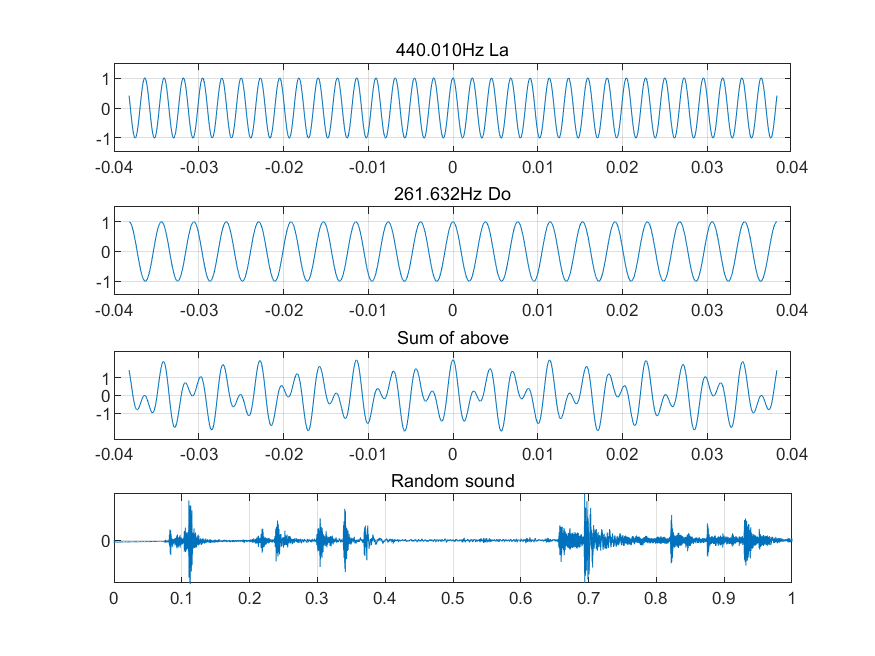
\includegraphics[width=0.9\textwidth]{figure/fig_1.png}}
    \centerline{\textbf{Figure 1}}
  \end{minipage}
  \begin{minipage}{0.55\linewidth}
    \centerline{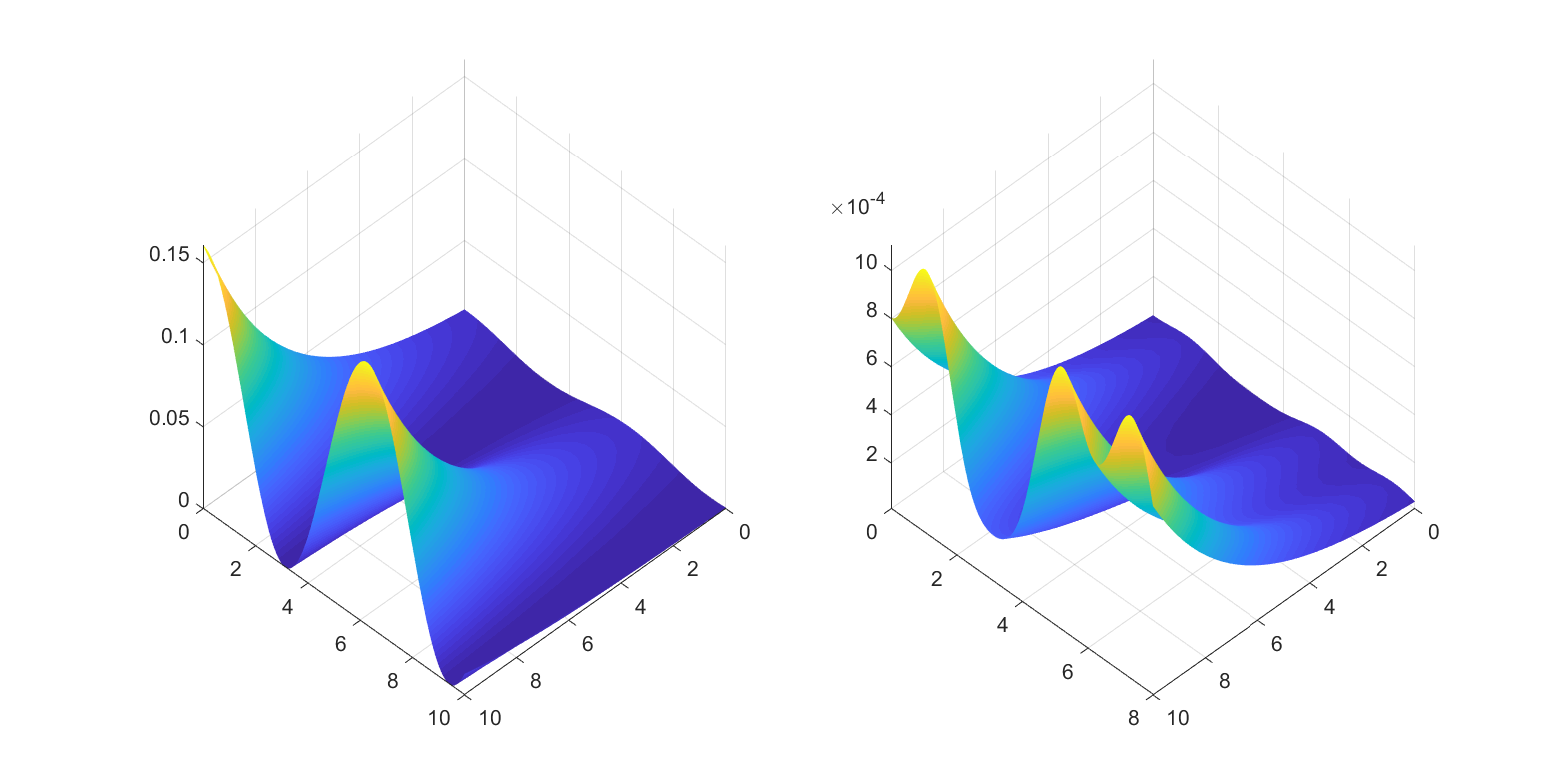
\includegraphics[width=\textwidth]{figure/fig_2.png}}
    \centerline{\textbf{Figure 2}}
  \end{minipage}
\end{figure}
In fact, many physical problems have the same properties, such as heat transfer problem. If we have a rod, which temperature function is $T=cos(x)$ .
The change of its temperature with time t presents a simple exponential decay form, as I showed in the first sub-graph of Figure 2.\par
But for a more complex temperature function $T=f(x)$ like the second sub-graph of Figure 2, if we can decompose it into the composition of a series sine and cosine function, we can simply migrate it to $T=F(x,t)$.\par
Let's start with simple one:a sinusoidal signal of 4 beats per second. We can construct a rotating vector whose length is the same as this sinusoidal signal value of the current time. The graph of this vector will like the second sub-graph in Figure 3. We can find a magic phenomenon.When the frequency of this rotating vector is equal to this sinusoidal signal's frequency, a large number of points in this image are biased to the same side.\par
If we imagine this graph is having some kind of mass to it, like metal wire. We can find, as we change the frequency, the center of mass wobbles around a bit at origin. But when the frequency is equal to our signal frequency, the mass center is unusually far to the right. If we draw the x position of the mass center changed by the frequency into a $f-x$ graph. It will be like the third sub-figure in Figure 3. There is a high peak at 4 Hz position.\par
\begin{figure}[H]
	\begin{minipage}{0.48\linewidth}
		\centerline{\animategraphics[autoplay,loop,width=0.8\textwidth]{30}{figure/fig_3/fig-}{1}{601}}
		\centerline{\textbf{Figure 3}}
	\end{minipage}
	\begin{minipage}{0.48\linewidth}
		\centerline{\animategraphics[autoplay,loop,width=0.8\textwidth]{30}{figure/fig_4/fig-}{1}{601}}
		\centerline{\textbf{Figure 4}}
	\end{minipage}
\end{figure}
And we can do the same operation in a combination of two signal: $cos(2\pi 3t)+cos(2\pi 5t)$. Then we can get similar result: two peaks at 3 and 5 Hz. And now, we can make a bold assumptions that we can use the combination of sine or cosine signal to build another arbitrary signal. And we should proof it.\par
Let us assume $f(t)=\sum\limits^{N}A_n \cos (n\omega t+\phi)$, then

\begin{figure}[H]
	\centerline{\animategraphics[autoplay,loop,scale=0.5]{2}{figure/fig_5/fig-}{1}{10}}
\end{figure}
\clearpage

\section{\sc II. When the infinite sum has to be applied}
\clearpage

\section{\sc III. Open the gate to frequency domain}
\clearpage

\section{\sc IV. From periodicity to aperiodicity}
\clearpage

\end{resume}
\end{document}




